\def\TT{{\rm time}}
\def\SS{{\rm step}}

In this section, we present experimental evaluations that we performed to ensure the accuracy of the simulation code. 

\subsection{Accuracy of stencil operators}

In order to test the accuracy and convergence of WAMR and the derivative stencils, we used a known function to generate adaptive octree grid based on the wavelet expansion. 
Then we compute numerical derivatives using finite difference stencils which are compared against the analytical derivatives of $f(x,y,z)$. $l_2$ and $l_{\infty}$ norms of the comparison is given in the Table \ref{tb:fd}. 

\begin{table}
	\centering
	\scalebox{0.9}{
		\begin{tabular}{||c | c |c | c||} 
			\hline
			derivative & grid points & $\norm{.}_2$ & $\norm{.}_\infty$ \\
			\hline\hline
			$\partial_x$ & 4913 & 0.0201773 & 0.00144632 \\
			$\partial_x$ & 99221 & 0.000849063 & 2.74672e-05 \\
			\hline
		\end{tabular}
	}
	\caption{Normed difference in numerical derivative and analytical derivative evaluated at grid points for the function $f(x,y,z)=sin(2\pi x)sin(2\pi y)sin(2\pi z))$% \  (x,y,z)\in [-0.5,0.5]^3$ 
	where in both cases wavelet tolerance 
	of $10^{-8}$ but increasing maximum level of refinement (i.e. \texttt{maxDepth}) from $4$ to $6$. Note that when \texttt{maxDepth} increases number of grid points increase hence normed difference between numerical and analytical derivatives goes down significantly. }
	\label{tb:fd}
\end{table}





\subsection{Accuracy of symbolic interface and code generation}

Given the complexity of the \BSSN\ equations, writing code to
evaluate these equations can be an error-prone and tedious task.
For example, to evaluate the equations we need to calculate more than 300
finite derivatives. Hence \dendro\ provides a symbolic framework
written in \texttt{SymPy} for automatically generating C++ code for
the equations. The user writes equations in a high-level representation 
that more closely resembles their symbolic form. 
We can then use the computational graph
of the equations to generate optimized C++ code. The accuracy
of the symbolic framework and code generation is certified by comparing 
results from the generated C++ code to those from 
the \HAD\ code, an established and tested code for numerical relativity.

This table shows a comparison of \BSSN\ equations (i.e. all 24 equations),
evaluated over a grid of $128^3$ points by arbitrary, non-zero functions
by both the \dendro\ and \HAD\ codes. All spatial derivatives in the equations
are evaluated using finite differences, for both the
\dendro\ and \HAD\ codes.
The table reports the $L_2$ norm of the difference in the equations
as evaluated in both codes, 
as well as the $L_2$ norms of the functions used to evaluate the equations.
Equations with residual norms of order $10^{-15}$ are clearly at machine zero, 
but this low level is reached for only the simplest equations. Residuals with
norms of order $10^{-12}$ arise in complicated equations, where finite precision  
errors can accumulate in hundreds of floating point operations. The optimized
equations require about 4500 floating point operations to evaluate at a single point.

\begin{lstlisting}[basicstyle=\tiny]
L2 Norms differences in the HAD and DENDRO equations on 128^3 points.
------------------------------------------------------------------------
|| diff 0  || = 1.18413e-15, || rhs HAD || = 1.28114, || rhs DENDRO || = 1.28114
|| diff 1  || = 7.53412e-16, || rhs HAD || = 2.18877, || rhs DENDRO || = 2.18877
|| diff 2  || = 4.98271e-16, || rhs HAD || = 1.66315, || rhs DENDRO || = 1.66315
|| diff 3  || = 1.03346e-15, || rhs HAD || = 0.720477,|| rhs DENDRO || = 0.720477
|| diff 4  || = 5.82489e-16, || rhs HAD || = 1.40142, || rhs DENDRO || = 1.40142
|| diff 5  || = 4.93128e-16, || rhs HAD || = 0.797567,|| rhs DENDRO || = 0.797567
|| diff 6  || = 1.94194e-11, || rhs HAD || = 19.0107, || rhs DENDRO || = 19.0107
|| diff 7  || = 2.14958e-11, || rhs HAD || = 19.5221, || rhs DENDRO || = 19.5221
|| diff 8  || = 4.0673e-12,  || rhs HAD || = 8.96364, || rhs DENDRO || = 8.96364
|| diff 9  || = 1.58532e-11, || rhs HAD || = 10.1459, || rhs DENDRO || = 10.1459
|| diff 10 || = 4.31184e-12, || rhs HAD || = 8.70053, || rhs DENDRO || = 8.70053
|| diff 11 || = 4.95696e-12, || rhs HAD || = 10.8644, || rhs DENDRO || = 10.8644
|| diff 12 || = 4.27211e-15, || rhs HAD || = 19.3546, || rhs DENDRO || = 19.3546
|| diff 13 || = 2.29542e-10, || rhs HAD || = 93.4829, || rhs DENDRO || = 93.4829
|| diff 14 || = 1.7484e-11,  || rhs HAD || = 40.0804, || rhs DENDRO || = 40.0804
|| diff 15 || = 4.79216e-11, || rhs HAD || = 30.9279, || rhs DENDRO || = 30.9279
|| diff 16 || = 2.03434e-11, || rhs HAD || = 26.0603, || rhs DENDRO || = 26.0603
|| diff 17 || = 1.07479e-15, || rhs HAD || = 15.5765, || rhs DENDRO || = 15.5765
|| diff 18 || = 3.00151e-15, || rhs HAD || = 32.9891, || rhs DENDRO || = 32.9891
|| diff 19 || = 7.79103e-16, || rhs HAD || = 8.10107, || rhs DENDRO || = 8.10107
|| diff 20 || = 7.77113e-16, || rhs HAD || = 9.01369, || rhs DENDRO || = 9.01369
|| diff 21 || = 1.74839e-11, || rhs HAD || = 46.3141, || rhs DENDRO || = 46.3141
|| diff 22 || = 4.79217e-11, || rhs HAD || = 32.7981, || rhs DENDRO || = 32.7981
|| diff 23 || = 2.03434e-11, || rhs HAD || = 32.7256, || rhs DENDRO || = 32.7256
\end{lstlisting}

\subsection{Single black hole}
\label{sec:AE_sbh}

Prior to simulating binary inspirals, we perform simple experiments
with a single black hole to ensure the accuracy of the simulation code. 
While a single black hole is a stable, static solution of the Einstein 
equations, although there is some transient time dependence with:w
 our particular 
coordinate conditions.
%The key idea of the
%single black hole experiment is we make the mass of the one black
%hole comparably smaller and make it's initial placement far away
%from the second black hole, which makes the binary black hole system
%reduce to the single black hole, and since there is no any interaction
%solution of the single black hole should remain as same as the
%initial solution as we perform time stepping.  
The black hole
parameters (parameter file can be found in
\texttt{SC18\_AE/par/single\_bh1.par} in the repository) for this
test is given below. Note that to generate initial data for a single black
hole, we place one of the black holes in the binary far from the computational
domain and set its mass to zero.

\begin{lstlisting}[basicstyle=\small]
"BSSN_BH1": { "MASS":1.0, "X":0.0, "Y":0.0, 
"Z": 0.00123e-6, "V_X": 0.0, "V_Y": 0.0, 
"V_Z": 0.0, "SPIN": 0, 
"SPIN_THETA":0, "SPIN_PHI": 0 },

"BSSN_BH2": { "MASS":1e-15,"X":1e15, "Y":0.0, 
"Z":0.00123e-6, "V_X": 0.0, "V_Y": 0.0, 
"V_Z": 0.0, "SPIN": 0, 
"SPIN_THETA":0, "SPIN_PHI": 0 }
\end{lstlisting}


\begin{figure*}
	\begin{minipage}{0.32\linewidth}
		\subfloat[{$\SS=0,\ \TT=0~M$}] {
			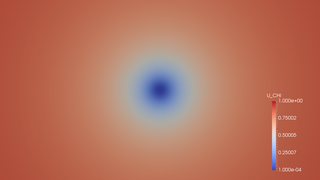
\includegraphics[width=0.8\textwidth]{figs/AE/sbh_boost/img_slice_000000.png}
		}
	\end{minipage}
	\begin{minipage}{0.32\linewidth}
		\subfloat[{$\SS=500,\ \TT=21.97~M$}] {
			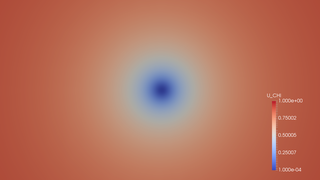
\includegraphics[width=0.8\textwidth]{figs/AE/sbh_boost/img_slice_000050.png}
		}
	\end{minipage}
	\begin{minipage}{0.32\linewidth}
		\subfloat[{$\SS=1000,\ \TT=43.94~M$}] {
			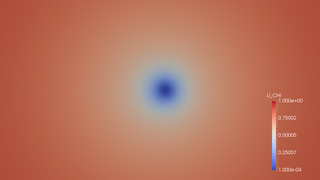
\includegraphics[width=0.8\textwidth]{figs/AE/sbh_boost/img_slice_000100.png}
		}
	\end{minipage} \hfill

	\begin{minipage}{0.32\linewidth}
			\subfloat[{$\SS=1500,\ \TT=65.91~M$}] {
				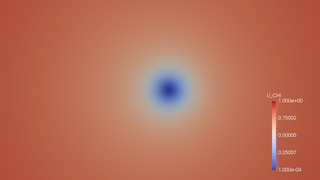
\includegraphics[width=0.8\textwidth]{figs/AE/sbh_boost/img_slice_000150.png}
			}
		\end{minipage}
		\begin{minipage}{0.32\linewidth}
			\subfloat[{$\SS=2000,\ \TT=87.88~M$}] {
				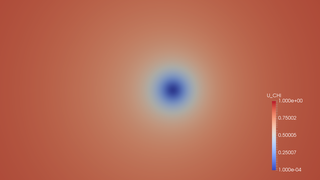
\includegraphics[width=0.8\textwidth]{figs/AE/sbh_boost/img_slice_000200.png}
			}
		\end{minipage}
		\begin{minipage}{0.32\linewidth}
			\subfloat[{$\SS=2500,\ \TT=109.85~M$}] {
				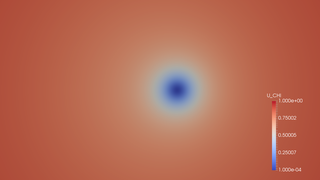
\includegraphics[width=0.8\textwidth]{figs/AE/sbh_boost/img_slice_000250.png}
			}
		\end{minipage} \hfill
	
	\begin{minipage}{0.32\linewidth}
		\subfloat[{$\SS=3000,\ \TT=131.82~M$}] {
			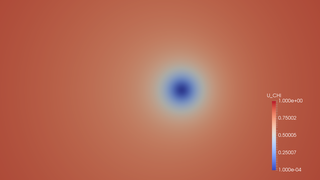
\includegraphics[width=0.8\textwidth]{figs/AE/sbh_boost/img_slice_000300.png}
		}
	\end{minipage}
	\begin{minipage}{0.32\linewidth}
		\subfloat[{$\SS=3500,\ \TT=153.79~M$}] {
			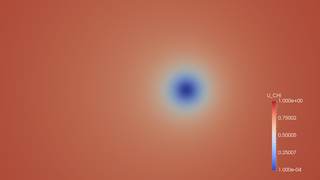
\includegraphics[width=0.8\textwidth]{figs/AE/sbh_boost/img_slice_000350.png}
		}
	\end{minipage}
	\begin{minipage}{0.32\linewidth}
		\subfloat[{$\SS=4000,\ \TT=175.76~M$}] {
			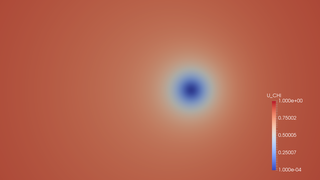
\includegraphics[width=0.8\textwidth]{figs/AE/sbh_boost/img_slice_000400.png}
		}
	\end{minipage} \hfill
	
	
	\begin{minipage}{0.32\linewidth}
		\subfloat[{$\SS=4500,\ \TT=197.73~M$}] {
			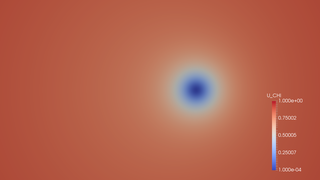
\includegraphics[width=0.8\textwidth]{figs/AE/sbh_boost/img_slice_000450.png}
	}
	\end{minipage}
	\begin{minipage}{0.32\linewidth}
		\subfloat[{$\SS=5000,\ \TT=219.70~M$}] {
			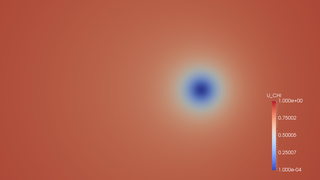
\includegraphics[width=0.8\textwidth]{figs/AE/sbh_boost/img_slice_000500.png}
		}
	\end{minipage}
	\begin{minipage}{0.32\linewidth}
		\subfloat[{$\SS=5500,\ \TT=241.67~M$}] {
			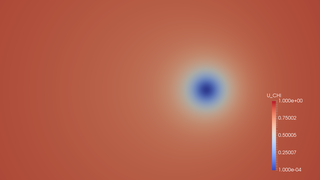
\includegraphics[width=0.8\textwidth]{figs/AE/sbh_boost/img_slice_000550.png}
	}
	\end{minipage} \hfill
	
		\begin{minipage}{0.32\linewidth}
			\subfloat[{$\SS=6000,\ \TT=263.64~M$}] {
				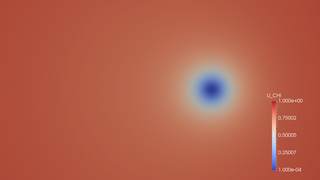
\includegraphics[width=0.8\textwidth]{figs/AE/sbh_boost/img_slice_000600.png}
			}
		\end{minipage}
		\begin{minipage}{0.32\linewidth}
			\subfloat[{$\SS=6500,\ \TT=285.61~M$}] {
				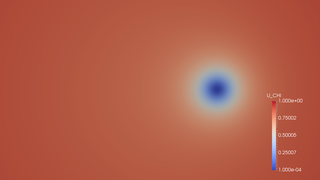
\includegraphics[width=0.8\textwidth]{figs/AE/sbh_boost/img_slice_000649.png}
			}
		\end{minipage} \hfill
%		\begin{minipage}{0.32\linewidth}
%			\subfloat[{$\SS=550$}] {
%				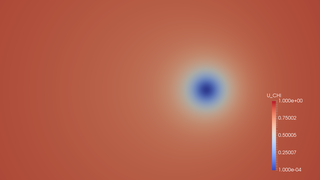
\includegraphics[width=0.8\textwidth]{figs/AE/sbh_boost/img_slice_000550.png}
%			}
%		\end{minipage} \hfill
	
	\caption{A single black hole boosted in the $x$-direction, with \maxDepth=12 and wavelet tolerance of $10^{-3}$. Time is given in terms of the black hole
mass, $M$. \label{fig:sbh_boost}}
\end{figure*}





\begin{figure*}
	\begin{minipage}{0.32\linewidth}
		\subfloat[{$\SS=0,\ \TT=0~M$}] {
			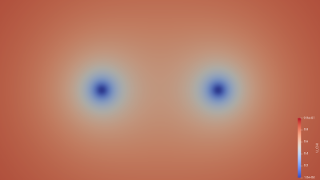
\includegraphics[width=0.8\textwidth]{figs/AE/r1/img_slice_000000.png}
		}
	\end{minipage}
	\begin{minipage}{0.32\linewidth}
		\subfloat[{$\SS=500,\ \TT=21.97~M$}] {
			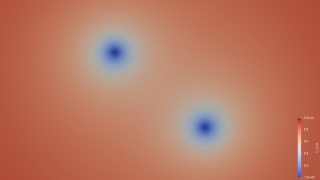
\includegraphics[width=0.8\textwidth]{figs/AE/r1/img_slice_000010.png}
		}
	\end{minipage}
	\begin{minipage}{0.32\linewidth}
		\subfloat[{$\SS=1000,\ \TT=43.94~M$}] {
			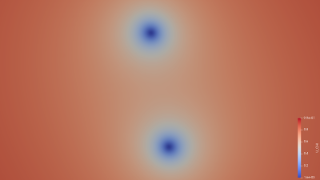
\includegraphics[width=0.8\textwidth]{figs/AE/r1/img_slice_000020.png}
		}
	\end{minipage} \hfill
	
	\begin{minipage}{0.32\linewidth}
		\subfloat[{$\SS=1500,\ \TT=65.91~M$}] {
			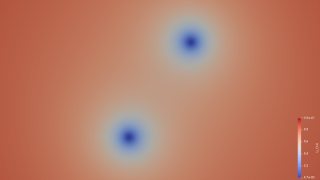
\includegraphics[width=0.8\textwidth]{figs/AE/r1/img_slice_000030.png}
		}
	\end{minipage}
	\begin{minipage}{0.32\linewidth}
		\subfloat[{$\SS=2000,\ \TT=87.88~M$}] {
			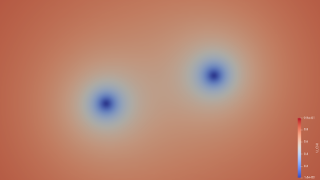
\includegraphics[width=0.8\textwidth]{figs/AE/r1/img_slice_000040.png}
		}
	\end{minipage}
	\begin{minipage}{0.32\linewidth}
		\subfloat[{$\SS=2500,\ \TT=109.85~M$}] {
			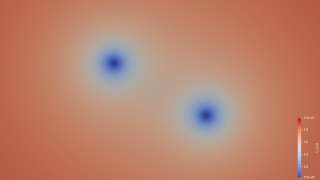
\includegraphics[width=0.8\textwidth]{figs/AE/r1/img_slice_000050.png}
		}
	\end{minipage} \hfill
	
	\begin{minipage}{0.32\linewidth}
		\subfloat[{$\SS=3000,\ \TT=131.82~M$}] {
			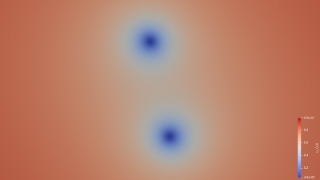
\includegraphics[width=0.8\textwidth]{figs/AE/r1/img_slice_000060.png}
		}
	\end{minipage}
	\begin{minipage}{0.32\linewidth}
		\subfloat[{$\SS=3500,\ \TT=153.79~M$}] {
			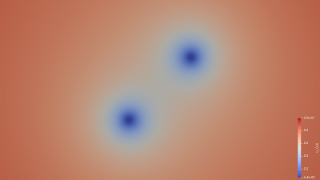
\includegraphics[width=0.8\textwidth]{figs/AE/r1/img_slice_000070.png}
		}
	\end{minipage}
	\begin{minipage}{0.32\linewidth}
		\subfloat[{$\SS=4000,\ \TT=175.76~M$}] {
			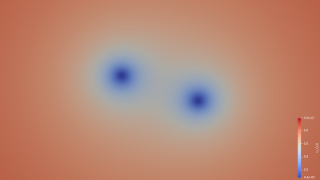
\includegraphics[width=0.8\textwidth]{figs/AE/r1/img_slice_000080.png}
		}
	\end{minipage} \hfill
	
	
	\begin{minipage}{0.32\linewidth}
		\subfloat[{$\SS=4500,\ \TT=197.73~M$}] {
			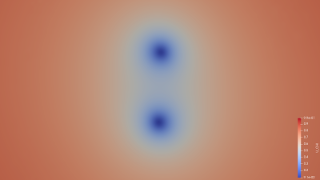
\includegraphics[width=0.8\textwidth]{figs/AE/r1/img_slice_000090.png}
		}
	\end{minipage}
	\begin{minipage}{0.32\linewidth}
		\subfloat[{$\SS=5000,\ \TT=219.70~M$}] {
			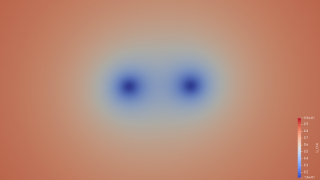
\includegraphics[width=0.8\textwidth]{figs/AE/r1/img_slice_000100.png}
		}
	\end{minipage}
	\begin{minipage}{0.32\linewidth}
		\subfloat[{$\SS=5500,\ \TT=241.67~M$}] {
			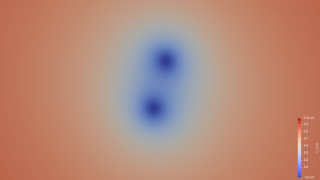
\includegraphics[width=0.8\textwidth]{figs/AE/r1/img_slice_000110.png}
		}
	\end{minipage} \hfill

	\caption{This figure shows frames from the evolution of a black hole
binary with an equal mass ratio, $q=1$. Time is measured in terms of the total
black hole mass $M$.\label{fig:r1}	}
\end{figure*}


\begin{figure*}
	\begin{minipage}{0.32\linewidth}
		\subfloat[{$\SS=0,\ \TT=0~M$}] {
			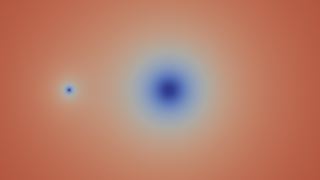
\includegraphics[width=0.8\textwidth]{figs/AE/r10/img_slice_000000.png}
		}
	\end{minipage}
	\begin{minipage}{0.32\linewidth}
		\subfloat[{$\SS=500,\ \TT=21.97~M$}] {
			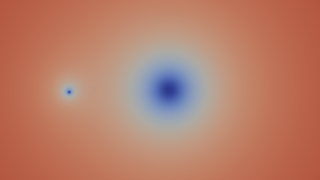
\includegraphics[width=0.8\textwidth]{figs/AE/r10/img_slice_000010.png}
		}
	\end{minipage}
	\begin{minipage}{0.32\linewidth}
		\subfloat[{$\SS=1000,\ \TT=43.94~M$}] {
			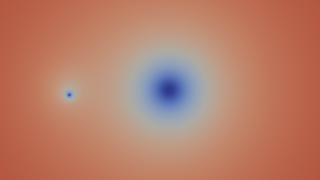
\includegraphics[width=0.8\textwidth]{figs/AE/r10/img_slice_000020.png}
		}
	\end{minipage} \hfill
	
	\begin{minipage}{0.32\linewidth}
		\subfloat[{$\SS=1500,\ \TT=65.91~M$}] {
			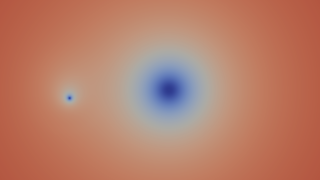
\includegraphics[width=0.8\textwidth]{figs/AE/r10/img_slice_000030.png}
		}
	\end{minipage}
	\begin{minipage}{0.32\linewidth}
		\subfloat[{$\SS=2000,\ \TT=87.88~M$}] {
			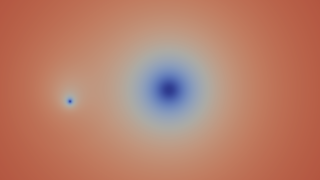
\includegraphics[width=0.8\textwidth]{figs/AE/r10/img_slice_000040.png}
		}
	\end{minipage}
	\begin{minipage}{0.32\linewidth}
		\subfloat[{$\SS=2500,\ \TT=109.85~M$}] {
			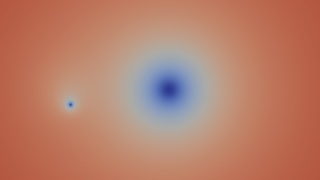
\includegraphics[width=0.8\textwidth]{figs/AE/r10/img_slice_000050.png}
		}
	\end{minipage} \hfill
	
	\begin{minipage}{0.32\linewidth}
		\subfloat[{$\SS=3000,\ \TT=131.82~M$}] {
			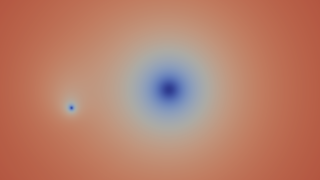
\includegraphics[width=0.8\textwidth]{figs/AE/r10/img_slice_000060.png}
		}
	\end{minipage}
	\begin{minipage}{0.32\linewidth}
		\subfloat[{$\SS=3500,\ \TT=153.79~M$}] {
			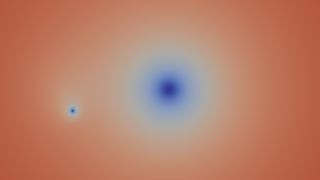
\includegraphics[width=0.8\textwidth]{figs/AE/r10/img_slice_000070.png}
		}
	\end{minipage}
	\begin{minipage}{0.32\linewidth}
		\subfloat[{$\SS=4000,\ \TT=175.76~M$}] {
			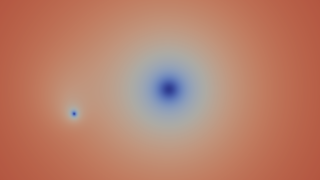
\includegraphics[width=0.8\textwidth]{figs/AE/r10/img_slice_000080.png}
		}
	\end{minipage} \hfill
	
	
	\begin{minipage}{0.32\linewidth}
		\subfloat[{$\SS=4500,\ \TT=197.73~M$}] {
			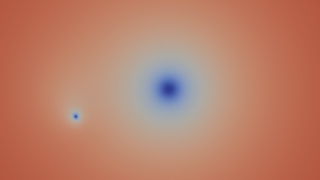
\includegraphics[width=0.8\textwidth]{figs/AE/r10/img_slice_000090.png}
		}
	\end{minipage}
	\begin{minipage}{0.32\linewidth}
		\subfloat[{$\SS=5000,\ \TT=219.70~M$}] {
			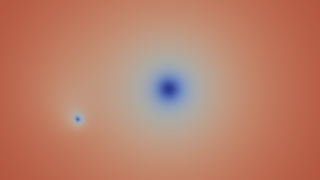
\includegraphics[width=0.8\textwidth]{figs/AE/r10/img_slice_000100.png}
		}
	\end{minipage}
	\begin{minipage}{0.32\linewidth}
		\subfloat[{$\SS=5500,\ \TT=241.67~M$}] {
			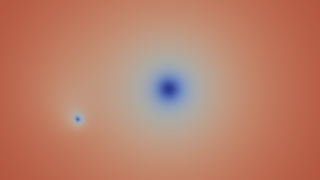
\includegraphics[width=0.8\textwidth]{figs/AE/r10/img_slice_000100.png}
		}
	\end{minipage} \hfill
	

	\caption{This figure shows frames from the evolution of a black hole
binary with mass ratio $q=10$. Time is measured in terms of the total
black hole mass $M$.\label{fig:r10}}
\end{figure*}




\begin{figure*}
	\begin{minipage}{0.32\linewidth}
		\subfloat[{$\SS=0,\ \TT=0~M$}] {
			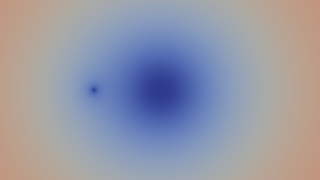
\includegraphics[width=0.8\textwidth]{figs/AE/r100/img_slice_000000.png}
		}
	\end{minipage}
	\begin{minipage}{0.32\linewidth}
		\subfloat[{$\SS=500,\ \TT=21.97~M$}] {
			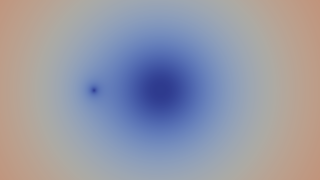
\includegraphics[width=0.8\textwidth]{figs/AE/r100/img_slice_000020.png}
		}
	\end{minipage}
	\begin{minipage}{0.32\linewidth}
		\subfloat[{$\SS=1000,\ \TT=43.94~M$}] {
			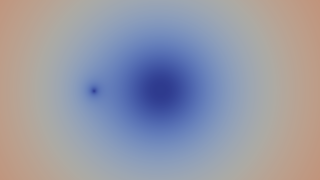
\includegraphics[width=0.8\textwidth]{figs/AE/r100/img_slice_000040.png}
		}
	\end{minipage} \hfill

	\begin{minipage}{0.32\linewidth}
		\subfloat[{$\SS=1500,\ \TT=65.91~M$}] {
			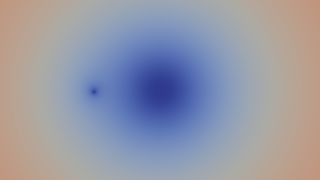
\includegraphics[width=0.8\textwidth]{figs/AE/r100/img_slice_000060.png}
		}
	\end{minipage} 
	\begin{minipage}{0.32\linewidth}
		\subfloat[{$\SS=2000,\ \TT=87.88~M$}] {
			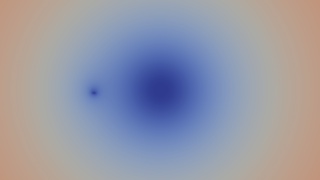
\includegraphics[width=0.8\textwidth]{figs/AE/r100/img_slice_000080.png}
		}
	\end{minipage}
	\begin{minipage}{0.32\linewidth}
		\subfloat[{$\SS=2500,\ \TT=109.85~M$}] {
			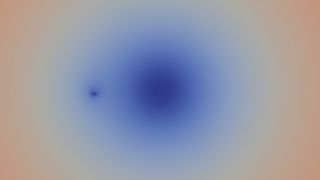
\includegraphics[width=0.8\textwidth]{figs/AE/r100/img_slice_000100.png}
		}
	\end{minipage} \hfill

	\begin{minipage}{0.32\linewidth}
		\subfloat[{$\SS=3000,\ \TT=131.82~M$}] {
			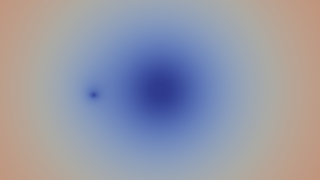
\includegraphics[width=0.8\textwidth]{figs/AE/r100/img_slice_000120.png}
		}
	\end{minipage}
	\begin{minipage}{0.32\linewidth}
		\subfloat[{$\SS=3500,\ \TT=153.79~M$}] {
			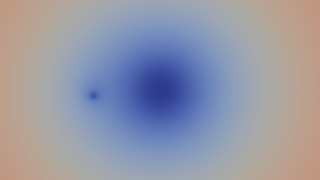
\includegraphics[width=0.8\textwidth]{figs/AE/r100/img_slice_000140.png}
		} 
	\end{minipage} 
	\begin{minipage}{0.32\linewidth}
		\subfloat[{$\SS=4000,\ \TT=175.76~M$}] {
			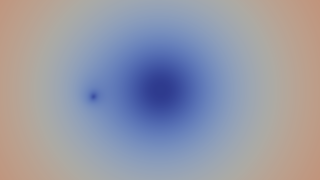
\includegraphics[width=0.8\textwidth]{figs/AE/r100/img_slice_000160.png}
		}
	\end{minipage} \hfill

	\begin{minipage}{0.32\linewidth}
		\subfloat[{$\SS=4500,\ \TT=197.73~M$}] {
			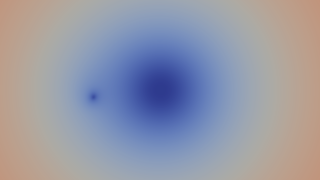
\includegraphics[width=0.8\textwidth]{figs/AE/r100/img_slice_000180.png}
		}
	\end{minipage}
	\begin{minipage}{0.32\linewidth}
		\subfloat[{$\SS=5000,\ \TT=219.70~M$}] {
			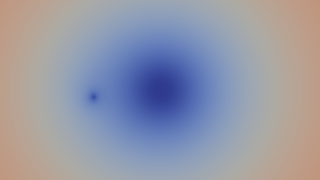
\includegraphics[width=0.8\textwidth]{figs/AE/r100/img_slice_000200.png}
		}
	\end{minipage}
	\begin{minipage}{0.32\linewidth}
		\subfloat[{$\SS=5500,\ \TT=241.67~M$}] {
			\includegraphics[width=0.8\textwidth]{figs/AE/r100/img_slice_000220.png}
		}
	\end{minipage}\hfill
 
	\caption{This figure shows frames from the evolution of a black hole binary 
with mass ratio $q=100$. Time is given
in terms of the total mass $M$.\label{fig:r100}}
\end{figure*}











\subsection{Boosted Single Black Hole}
\label{sec:AE_sbhboost}

The next experiment is an extension of the single BH test;
it ``boosts'' the BH with constant velocity in $x$-direction.
The constant velocity of the BH should be apparent in the evolution. 
The parameter file for this test can be found in the repository at 
\texttt{SC18\_AE/par/single\_bh1\_boost.par}.
The black hole parameters are given below (note
that $BSSN\_BH1$ has a momentum of 0.114 in $x$-direction).

\begin{lstlisting}[basicstyle=\small]
"BSSN_BH1": { "MASS":1.0, "X":0.0, "Y":0.0, 
"Z": 0.00123e-6, "V_X": 0.114, "V_Y": 0.0, 
"V_Z": 0.0, "SPIN": 0, 
"SPIN_THETA":0, "SPIN_PHI": 0 },

"BSSN_BH2": { "MASS":1e-15,"X":1e15, "Y":0.0, 
"Z":0.00123e-6, "V_X": 0.0, "V_Y": 0.0, 
"V_Z": 0.0, "SPIN": 0, 
"SPIN_THETA":0, "SPIN_PHI": 0 }
\end{lstlisting}



\subsection{Constraint equations}

Similar to the Maxwell equations of electrodynamics, the Einstein equations
contain both hyperbolic evolution equations and elliptic constraint equations,
which must be satisfied at all times. Following the common practice in
numerical relativity, we evolve the hyperbolic equations and monitor the 
quality of the solution by checking that the constraint equations are 
satisfied. The choice of coordinates for the BBH evolution (the puncture gauge) 
does induce constraint violations in the vicinity of each black hole.
The violations of the constraint equations in our runs are consistent with 
the discretization error expected for the numerical derivatives in the
constraint equations and the constraint violations near the black holes 
(punctures). An example of monitored constraint violations are listed in the Table \ref{tb:constraints}.

\begin{table}
	\centering
\scalebox{0.9}{
	\begin{tabular}{||c | c | c | c| c||} 
		\hline
		Time (M) & $\norm{\mathcal{H}_{r>a}}_2$ & $\norm{M1_{r>a}}_2$ & $\norm{M2_{r>a}}_2$ & $\norm{M3_{r>a}}_2$ \\
		\hline\hline
		0 & 0.000777861 & 1.01855e-05 & 1.23443e-05 & 7.17572e-06 \\
		0.976562 & 0.000808294 & 3.05681e-05 & 2.91217e-05 & 2.79631e-05 \\
		1.95312 & 0.000793783 & 5.03912e-05 & 3.93872e-05 & 4.06693e-05 \\
		2.92969 & 0.00079551 & 7.54643e-05 & 5.068e-05 & 5.42466e-05 \\
		3.90625	& 0.000956987 & 0.000102901 & 7.38208e-05 & 7.47156e-05 \\
		4.88281 & 0.00247348 & 0.000200055	& 0.000140583 & 0.000139008 \\
		\hline
	\end{tabular}
}
\caption{Violation of constraint equations with time for an equal mass ratio binary merger simulation done using OT. Note that $\mathcal{H}$, $M1,M2,M3$ denotes the Hamiltonian \& 3 momentum component constraints that is being monitored through the evolution.}
\label{tb:constraints}
\end{table}





\subsection{Binary black holes with mass ratio $q=1$}

We performed a series of short-term binary BH evolutions with different
mass ratios. This run was used to validate the code by comparing the
trajectories of the BHs calculated using \dendro\ to the trajectories calculated
by \HAD. Frames from the evolution are shown in the Figure~\ref{fig:r1},
%the figure,
and the BH parameters used for this run are listed below.

\begin{lstlisting}[basicstyle=\small]
  "BSSN_BH1": {
    "MASS":0.485,
    "X": 4.00e+00, "Y":0.0, "Z": 1.41-05,
    "V_X": -0.00133, "V_Y": 0.112, "V_Z": 0,
    "SPIN": 0, "SPIN_THETA":0, "SPIN_PHI": 0 },
  "BSSN_BH2": {
      "MASS":0.485,
      "X":-4.00+00, "Y":0.0, "Z":1.41-05,
      "V_X": 0.00132, "V_Y": -0.112, "V_Z": 0,
      "SPIN": 0, "SPIN_THETA":0, "SPIN_PHI": 0 }
\end{lstlisting}


\subsection{Binary black holes with mass ratio $q=10$}

We performed a short simulation with a mass ratio $q=10$
This is a short demonstration run to show that \dendro\
easily handles large mass ratios and gives consistent
results for the binary evolution.
Frames from the evolution are shown in figure,
and the BH parameters used for this run are listed below.

\begin{lstlisting}[basicstyle=\small]
  "BSSN_BH1": {
    "MASS":0.903,
    "X":5.45-01, "Y":0.0, "Z": 1.41-05,
    "V_X": -3.90e-04, "V_Y": 0.0470, "V_Z": 0,
    "SPIN": 0, "SPIN_THETA":0, "SPIN_PHI": 0 },
  "BSSN_BH2": {
      "MASS":0.0845,
      "X":-5.45+00, "Y":0.0, "Z":1.41-05,
      "V_X": 3.90e-04, "V_Y": -0.0470, "V_Z": 0,
      "SPIN": 0, "SPIN_THETA":0, "SPIN_PHI": 0 }
\end{lstlisting}

\subsection{Binary black holes with mass ratio $q=100$}

We performed a short simulation with a mass ratio $q=100$
This is a short demonstration run to show that \dendro\ 
produces the proper grid structure for this system and
reasonable results for a very challenging binary configuration.
Frames from the evolution are shown in the figure
and the BH parameters used for this run are listed below.


\begin{lstlisting}[basicstyle=\small]
  "BSSN_BH1": {
    "MASS":0.989,
    "X":5.94-02, "Y":0.0, "Z": 1.41-05,
    "V_X": -5.60-06, "V_Y": 5.61-03, "V_Z": 0,
    "SPIN": 0, "SPIN_THETA":0, "SPIN_PHI": 0 },
  "BSSN_BH2": {
      "MASS":0.00914,
      "X":-5.94+00, "Y":0.0, "Z":1.41421356e-05,
      "V_X": 5.60-06, "V_Y": -5.61-03, "V_Z": 0,
      "SPIN": 0, "SPIN_THETA":0, "SPIN_PHI": 0 }
\end{lstlisting}
